\documentclass[10pt,a4paper,twocolumn]{jarticle}
%
\usepackage[margin=20mm]{geometry}
\usepackage{amsmath,amssymb}
\usepackage{bm}
\usepackage{booktabs}
\usepackage[dvipdfmx]{graphicx}
\usepackage{longtable}
\usepackage[dvipdfm]{hyperref}


\makeatletter
\def\tightlist{\itemsep1pt\parskip0pt\parsep0pt}

\def\@maketitle{
\begin{flushright}
  $if(date)$ $date$ $endif$
\end{flushright}

\begin{flushleft}
{\large \bf $if(thesis)$ $thesis$ $endif$ \par} %演習
{\bf 題 目: $if(title)$ $title$$endif$ \par }% 論文のタイトル
{    \bf $if(titleE)$ $titleE$ $endif$ \par}
{\bf 発表者:$if(author)$ $author$ $endif$ \par }% 発表者
{    \bf $if(authorE)$ $authorE$ $endif$ \par }% 発表者
{\bf 所 属:$if(labo)$ $labo$ $endif$ \par }	% 所属
{    \bf $if(laboE)$ $laboE$ $endif$ }

\end{flushleft}
}

\makeatother

\makeatletter
\def\maxwidth{\ifdim\Gin@nat@width>\linewidth\linewidth\else\Gin@nat@width\fi}
\def\maxheight{\ifdim\Gin@nat@height>\textheight\textheight\else\Gin@nat@height\fi}
\makeatother
\setkeys{Gin}{width=\maxwidth,height=\maxheight,keepaspectratio}

\renewcommand{\abstractname}{\normalsize Abstract}


\begin{document}
    \twocolumn[
    \begin{@twocolumnfalse}
      \maketitle
      \begin{abstract}
        This is Abstract . WOOW. d

      \end{abstract}
    \end{@twocolumnfalse}
  ]

  %  \documentclass[10pt,a4paper,twocolumn]{jarticle}
%
\usepackage[margin=20mm]{geometry}
\usepackage{amsmath,amssymb}
\usepackage{bm}
\usepackage{booktabs}
\usepackage[dvipdfmx]{graphicx}
\usepackage{longtable}
\usepackage[dvipdfm]{hyperref}


\makeatletter
\def\tightlist{\itemsep1pt\parskip0pt\parsep0pt}

\def\@maketitle{
\begin{flushright}
   20XX/X/X G会場 
\end{flushright}

\begin{flushleft}
{\large \bf  XXXXX特別演習  \par} %演習
{\bf 題 目:  タイトル \par }% 論文のタイトル
{    \bf  Title  \par}
{\bf 発表者: 発表者名  \par }% 発表者
{    \bf  Author Name  \par }% 発表者
{\bf 所 属: XXXX~研究室( XXXX研)  \par }	% 所属
{    \bf  AAAA lab.(XXXX lab.)  }

\end{flushleft}
}

\makeatother

\makeatletter
\def\maxwidth{\ifdim\Gin@nat@width>\linewidth\linewidth\else\Gin@nat@width\fi}
\def\maxheight{\ifdim\Gin@nat@height>\textheight\textheight\else\Gin@nat@height\fi}
\makeatother
\setkeys{Gin}{width=\maxwidth,height=\maxheight,keepaspectratio}

\renewcommand{\abstractname}{\normalsize Abstract}


\begin{document}
    \twocolumn[
    \begin{@twocolumnfalse}
      \maketitle
      \begin{abstract}
        This is Abstract . WOOW. d

      \end{abstract}
    \end{@twocolumnfalse}
  ]

  %  \documentclass[10pt,a4paper,twocolumn]{jarticle}
%
\usepackage[margin=20mm]{geometry}
\usepackage{amsmath,amssymb}
\usepackage{bm}
\usepackage{booktabs}
\usepackage[dvipdfmx]{graphicx}
\usepackage{longtable}
\usepackage[dvipdfm]{hyperref}


\makeatletter
\def\tightlist{\itemsep1pt\parskip0pt\parsep0pt}

\def\@maketitle{
\begin{flushright}
   20XX/X/X G会場 
\end{flushright}

\begin{flushleft}
{\large \bf  XXXXX特別演習  \par} %演習
{\bf 題 目:  タイトル \par }% 論文のタイトル
{    \bf  Title  \par}
{\bf 発表者: 発表者名  \par }% 発表者
{    \bf  Author Name  \par }% 発表者
{\bf 所 属: XXXX~研究室( XXXX研)  \par }	% 所属
{    \bf  AAAA lab.(XXXX lab.)  }

\end{flushleft}
}

\makeatother

\makeatletter
\def\maxwidth{\ifdim\Gin@nat@width>\linewidth\linewidth\else\Gin@nat@width\fi}
\def\maxheight{\ifdim\Gin@nat@height>\textheight\textheight\else\Gin@nat@height\fi}
\makeatother
\setkeys{Gin}{width=\maxwidth,height=\maxheight,keepaspectratio}

\renewcommand{\abstractname}{\normalsize Abstract}


\begin{document}
    \twocolumn[
    \begin{@twocolumnfalse}
      \maketitle
      \begin{abstract}
        This is Abstract . WOOW. d

      \end{abstract}
    \end{@twocolumnfalse}
  ]

  %  \documentclass[10pt,a4paper,twocolumn]{jarticle}
%
\usepackage[margin=20mm]{geometry}
\usepackage{amsmath,amssymb}
\usepackage{bm}
\usepackage{booktabs}
\usepackage[dvipdfmx]{graphicx}
\usepackage{longtable}
\usepackage[dvipdfm]{hyperref}


\makeatletter
\def\tightlist{\itemsep1pt\parskip0pt\parsep0pt}

\def\@maketitle{
\begin{flushright}
   20XX/X/X G会場 
\end{flushright}

\begin{flushleft}
{\large \bf  XXXXX特別演習  \par} %演習
{\bf 題 目:  タイトル \par }% 論文のタイトル
{    \bf  Title  \par}
{\bf 発表者: 発表者名  \par }% 発表者
{    \bf  Author Name  \par }% 発表者
{\bf 所 属: XXXX~研究室( XXXX研)  \par }	% 所属
{    \bf  AAAA lab.(XXXX lab.)  }

\end{flushleft}
}

\makeatother

\makeatletter
\def\maxwidth{\ifdim\Gin@nat@width>\linewidth\linewidth\else\Gin@nat@width\fi}
\def\maxheight{\ifdim\Gin@nat@height>\textheight\textheight\else\Gin@nat@height\fi}
\makeatother
\setkeys{Gin}{width=\maxwidth,height=\maxheight,keepaspectratio}

\renewcommand{\abstractname}{\normalsize Abstract}


\begin{document}
    \twocolumn[
    \begin{@twocolumnfalse}
      \maketitle
      \begin{abstract}
        \input{abstract}
      \end{abstract}
    \end{@twocolumnfalse}
  ]

  %  \input {article}
  \hypertarget{ux306fux3058ux3081ux306b}{%
  \section{はじめに}\label{ux306fux3058ux3081ux306b}}
  
  Write Here Report
  
  二段組
  
  脚注{[}\^{}voodoo{]} 参考文献{[}1{]}.
  
  図.~\ref{fig:img}はラベル参照
  
  \begin{figure}
  \hypertarget{fig:img}{%
  \centering
  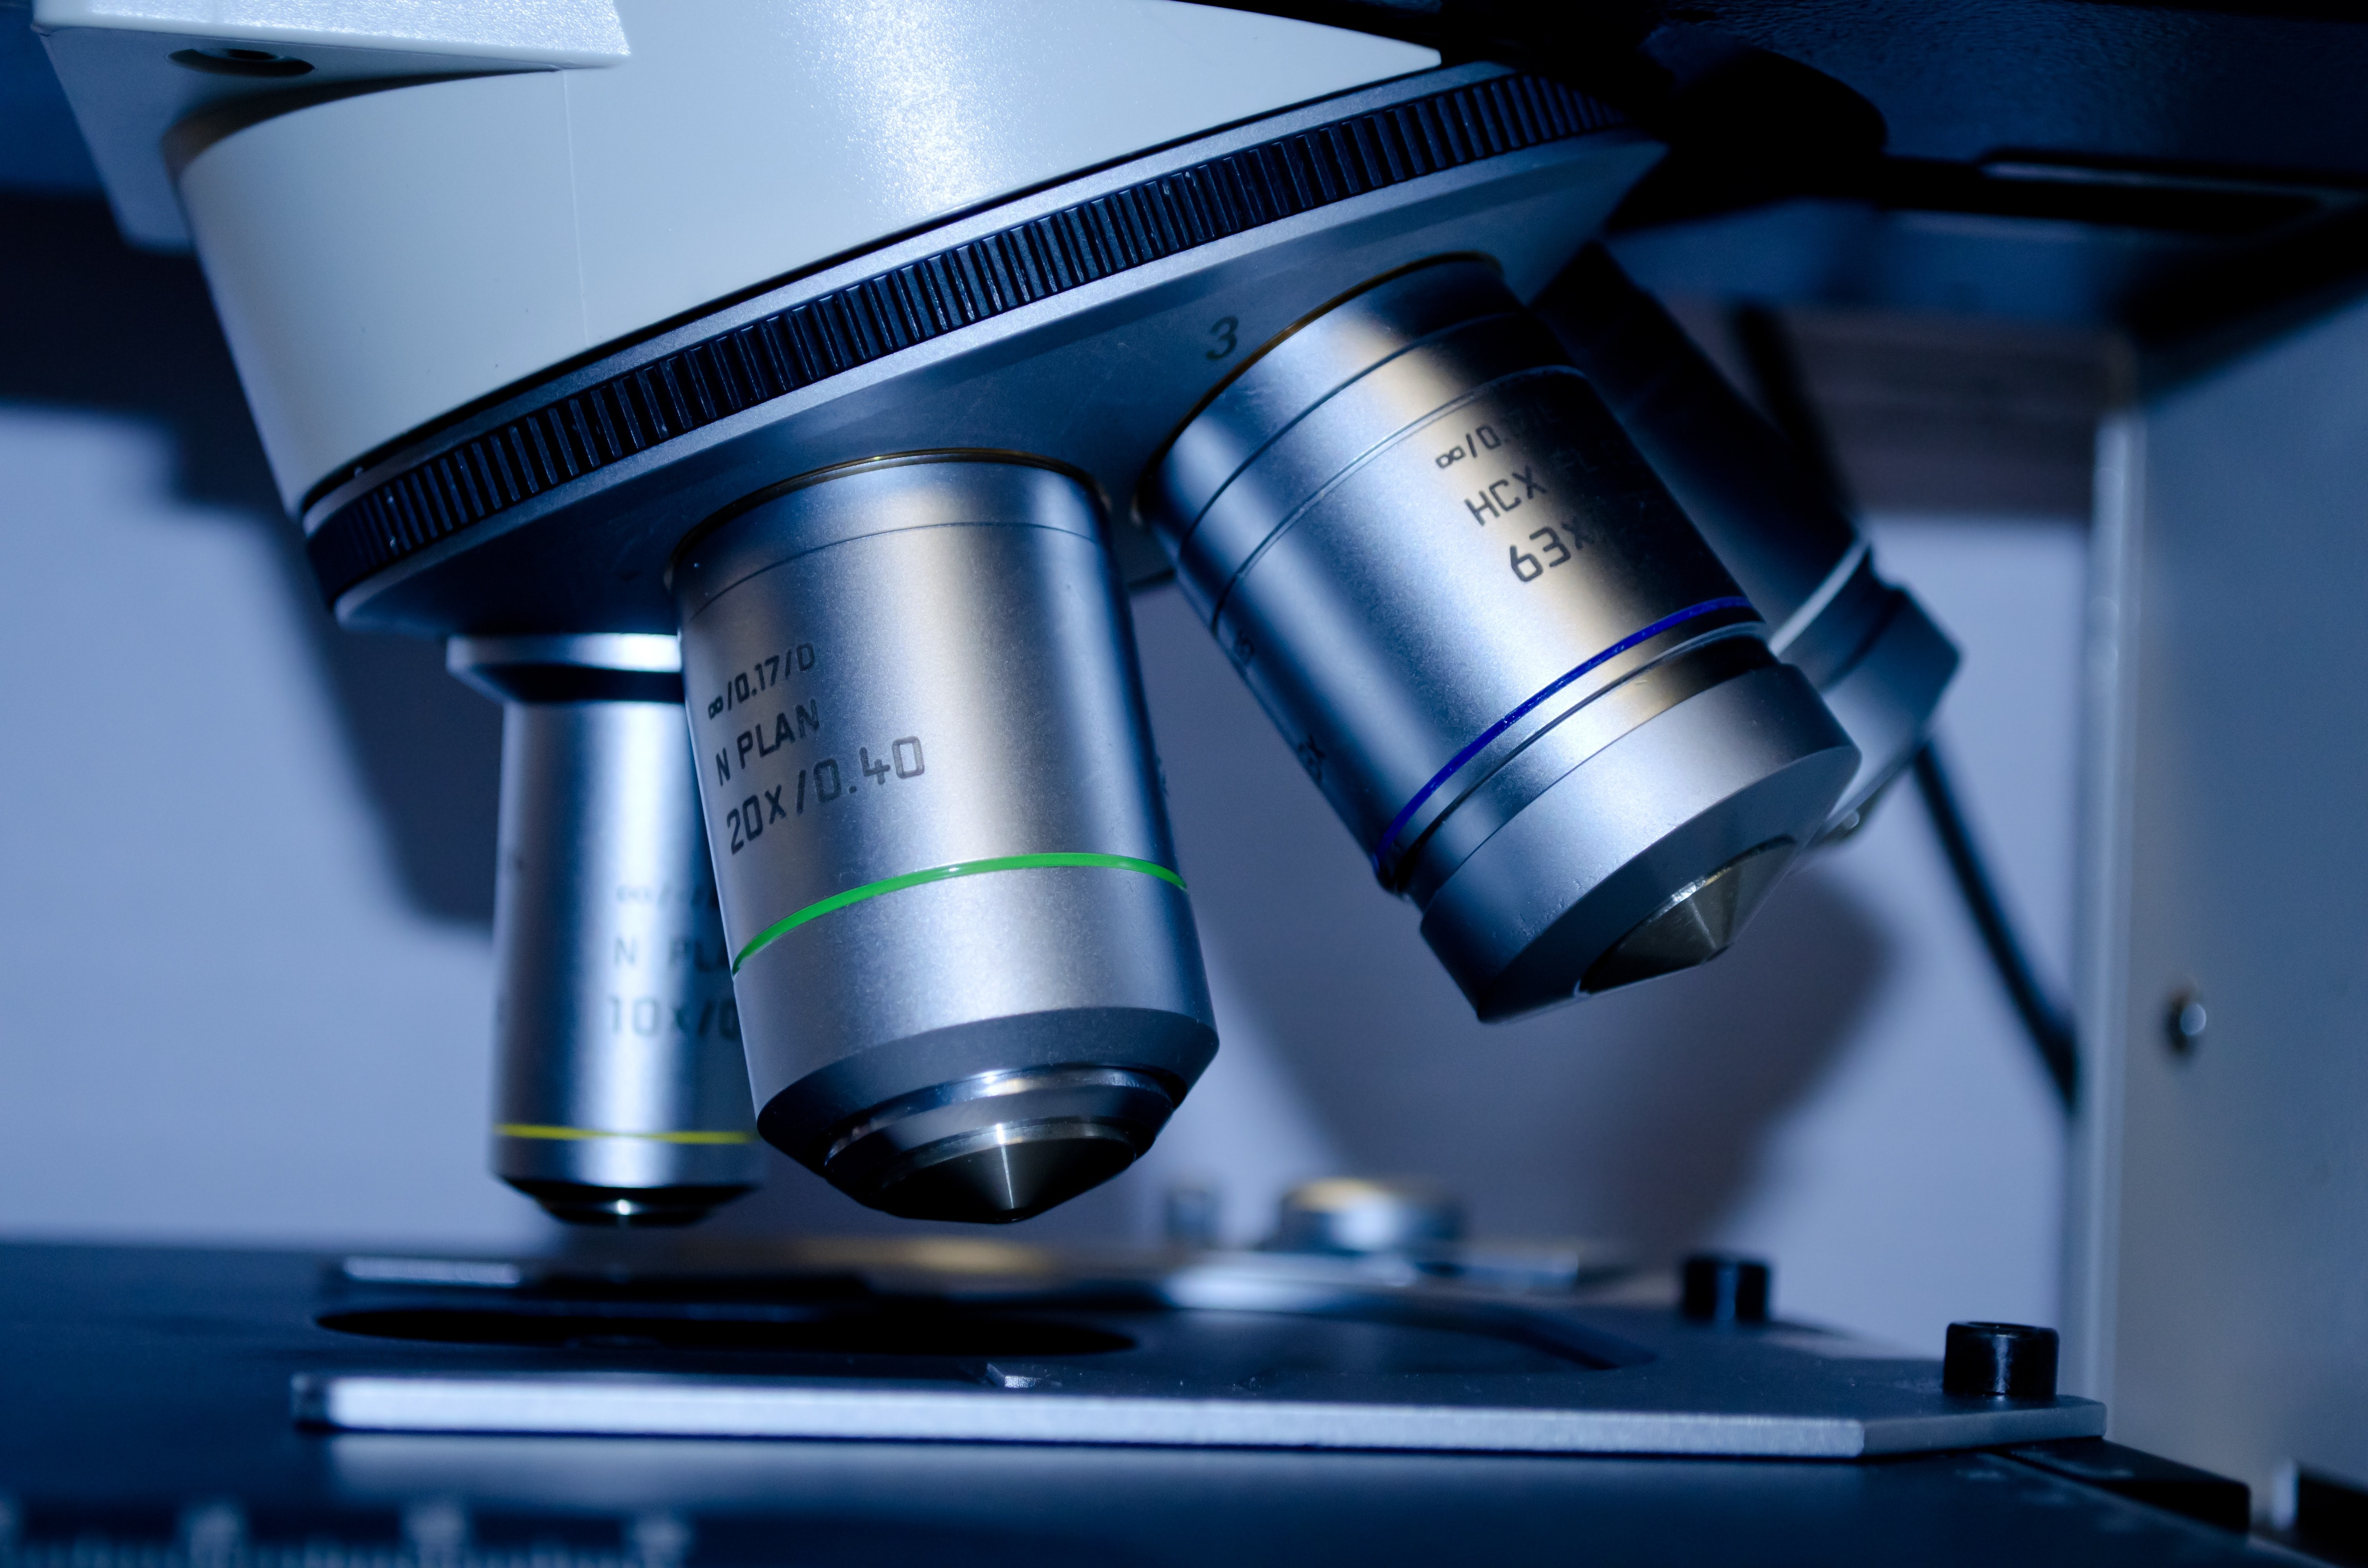
\includegraphics{img/img.jpg}
  \caption{キャプション}\label{fig:img}
  }
  \end{figure}
  
  \hypertarget{ux7ae0ux3068ux304b}{%
  \subsection{章とか}\label{ux7ae0ux3068ux304b}}
  
  \hypertarget{ux4ed6ux306e}{%
  \subsubsection{他の}\label{ux4ed6ux306e}}
  
    テスト
  
  表.~\ref{tbl:t} は表です.
  
  \hypertarget{tbl:t}{}
  \begin{table}[ht]
  \centering
  
  \caption{\label{tbl:t}キャプション}
  
  \begin{tabular}{@{}ll@{}}
  \toprule
  
  日常 & いいね \\\midrule
  
  起きる & 3 \\
  朝食をとる & 6 \\
  家を出る & 10 \\
  帰る      & 0 \\
  寝る & 0 \\
  
  \bottomrule
  \end{tabular}
  
  \end{table}
  
  式を式.~\ref{eq:eval}に示す.
  
  \begin{equation} Eq =  \frac{\sum_{i=0}^{n} (Y_i - X_i)} {n}  \label{eq:eval}\end{equation}
  
  \hypertarget{ux53c2ux8003ux6587ux732e}{%
  \section*{参考文献}\label{ux53c2ux8003ux6587ux732e}}
  \addcontentsline{toc}{section}{参考文献}
  
  \hypertarget{refs}{}
  \leavevmode\hypertarget{ref-ref}{}%
  {[}1{]} John Doe. 2016. \emph{Alan smithee}. OIMO Press. Retrieved from
  \url{http://www}

\bibliographystyle{junsrt}
\bibliography{reference}
\end{document}

  \hypertarget{ux306fux3058ux3081ux306b}{%
  \section{はじめに}\label{ux306fux3058ux3081ux306b}}
  
  Write Here Report
  
  二段組
  
  脚注{[}\^{}voodoo{]} 参考文献{[}1{]}.
  
  図.~\ref{fig:img}はラベル参照
  
  \begin{figure}
  \hypertarget{fig:img}{%
  \centering
  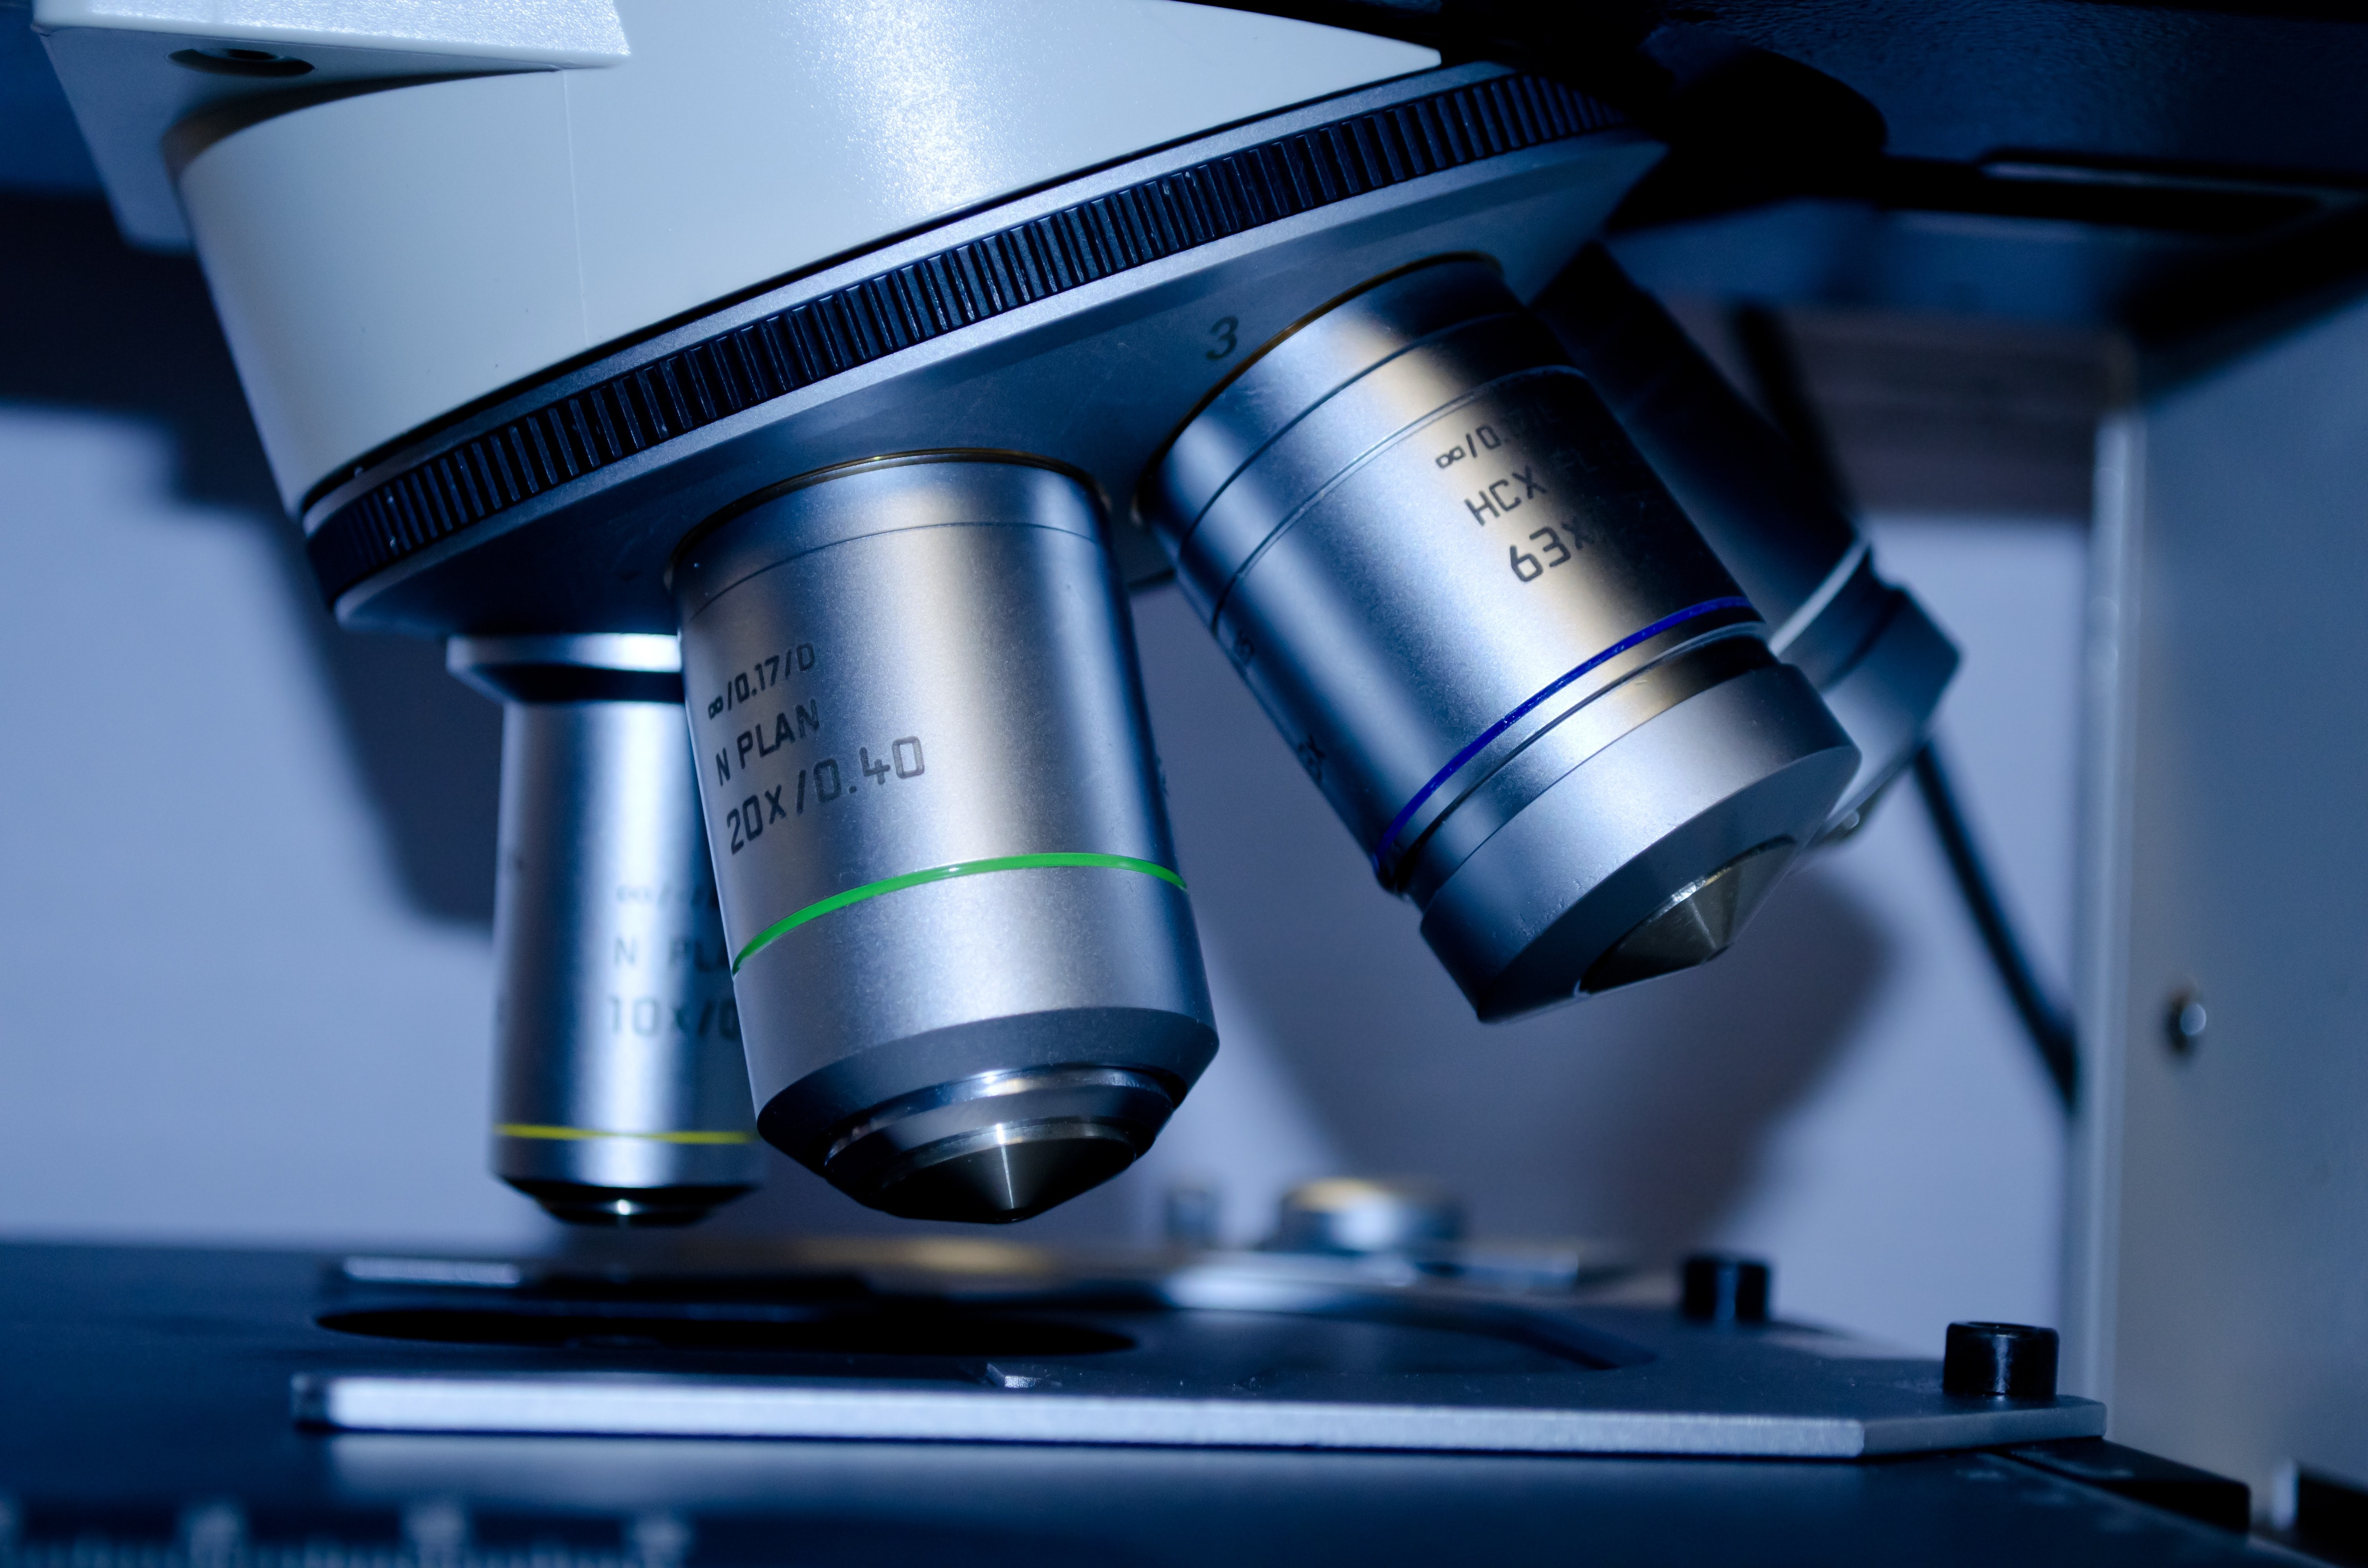
\includegraphics{img/img.jpg}
  \caption{キャプション}\label{fig:img}
  }
  \end{figure}
  
  \hypertarget{ux7ae0ux3068ux304b}{%
  \subsection{章とか}\label{ux7ae0ux3068ux304b}}
  
  \hypertarget{ux4ed6ux306e}{%
  \subsubsection{他の}\label{ux4ed6ux306e}}
  
    テスト
  
  表.~\ref{tbl:t} は表です.
  
  \hypertarget{tbl:t}{}
  \begin{table}[ht]
  \centering
  
  \caption{\label{tbl:t}キャプション}
  
  \begin{tabular}{@{}ll@{}}
  \toprule
  
  日常 & いいね \\\midrule
  
  起きる & 3 \\
  朝食をとる & 6 \\
  家を出る & 10 \\
  帰る      & 0 \\
  寝る & 0 \\
  
  \bottomrule
  \end{tabular}
  
  \end{table}
  
  式を式.~\ref{eq:eval}に示す.
  
  \begin{equation} Eq =  \frac{\sum_{i=0}^{n} (Y_i - X_i)} {n}  \label{eq:eval}\end{equation}
  
  \hypertarget{ux53c2ux8003ux6587ux732e}{%
  \section*{参考文献}\label{ux53c2ux8003ux6587ux732e}}
  \addcontentsline{toc}{section}{参考文献}
  
  \hypertarget{refs}{}
  \leavevmode\hypertarget{ref-ref}{}%
  {[}1{]} John Doe. 2016. \emph{Alan smithee}. OIMO Press. Retrieved from
  \url{http://www}

\bibliographystyle{junsrt}
\bibliography{reference}
\end{document}

  \hypertarget{ux306fux3058ux3081ux306b}{%
  \section{はじめに}\label{ux306fux3058ux3081ux306b}}
  
  Write Here Report
  
  二段組
  
  脚注{[}\^{}voodoo{]} 参考文献{[}1{]}.
  
  図.~\ref{fig:img}はラベル参照
  
  \begin{figure}
  \hypertarget{fig:img}{%
  \centering
  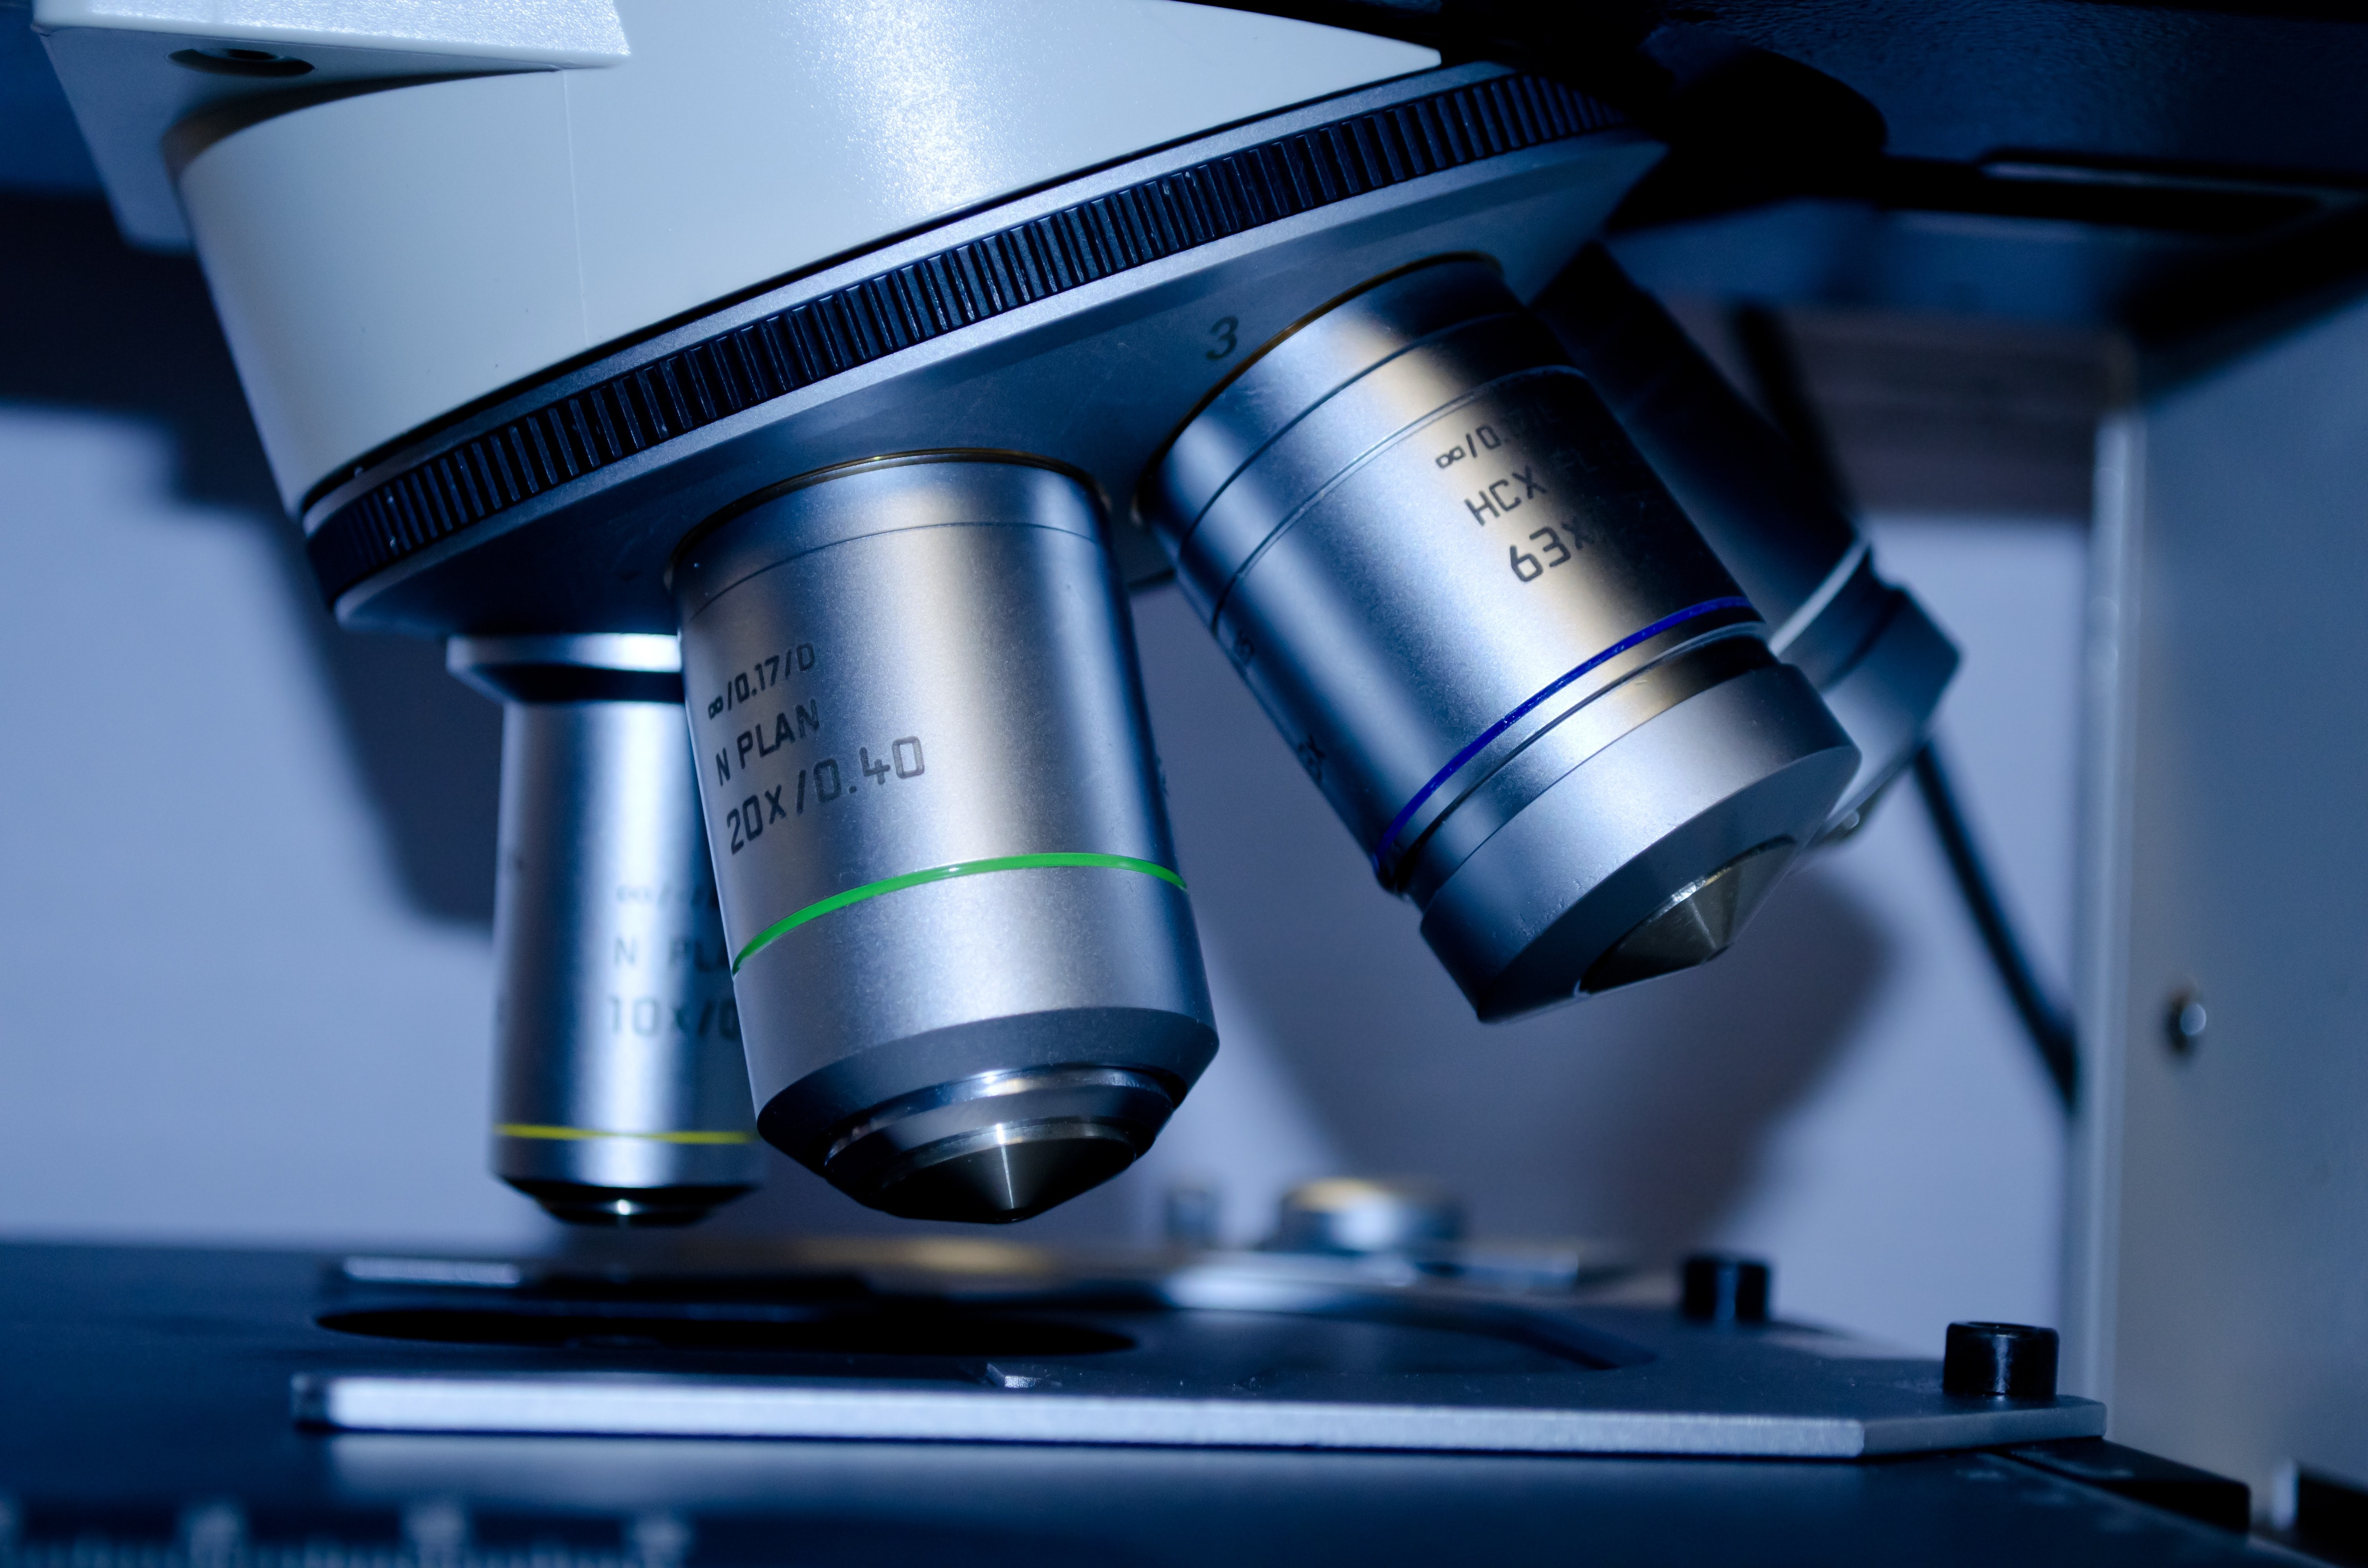
\includegraphics{img/img.jpg}
  \caption{キャプション}\label{fig:img}
  }
  \end{figure}
  
  \hypertarget{ux7ae0ux3068ux304b}{%
  \subsection{章とか}\label{ux7ae0ux3068ux304b}}
  
  \hypertarget{ux4ed6ux306e}{%
  \subsubsection{他の}\label{ux4ed6ux306e}}
  
    テスト
  
  表.~\ref{tbl:t} は表です.
  
  \hypertarget{tbl:t}{}
  \begin{table}[ht]
  \centering
  
  \caption{\label{tbl:t}キャプション}
  
  \begin{tabular}{@{}ll@{}}
  \toprule
  
  日常 & いいね \\\midrule
  
  起きる & 3 \\
  朝食をとる & 6 \\
  家を出る & 10 \\
  帰る      & 0 \\
  寝る & 0 \\
  
  \bottomrule
  \end{tabular}
  
  \end{table}
  
  式を式.~\ref{eq:eval}に示す.
  
  \begin{equation} Eq =  \frac{\sum_{i=0}^{n} (Y_i - X_i)} {n}  \label{eq:eval}\end{equation}
  
  \hypertarget{ux53c2ux8003ux6587ux732e}{%
  \section*{参考文献}\label{ux53c2ux8003ux6587ux732e}}
  \addcontentsline{toc}{section}{参考文献}
  
  \hypertarget{refs}{}
  \leavevmode\hypertarget{ref-ref}{}%
  {[}1{]} John Doe. 2016. \emph{Alan smithee}. OIMO Press. Retrieved from
  \url{http://www}

\bibliographystyle{junsrt}
\bibliography{reference}
\end{document}

  $body$

\bibliographystyle{junsrt}
\bibliography{reference}
\end{document}
